\documentclass[conference,,twocolumn]{IEEEtran}

\newcommand*{\MyPath}{../bib}
\usepackage{graphicx,psfrag,epsfig,epsf,latexsym,hhline,amsmath,amssymb,amsthm}
\usepackage{url}
\interdisplaylinepenalty=2500
\oddsidemargin =0.0in
\evensidemargin=0.0in
\topmargin=-0.1in
\headsep=0.0in
\textwidth=6.5in
\textheight=9.0in

\usepackage{psfrag,epsfig,epsf,latexsym,hhline,multirow}
\usepackage{tikz,pgfplots}
\usepgflibrary{plotmarks}
\pgfplotsset{compat=newest}
\pgfplotsset{plot coordinates/math parser=false}
\usetikzlibrary{arrows,shapes,chains,matrix,positioning,scopes,patterns}
\usetikzlibrary{decorations.markings}

\newlength\figureheight 
\newlength\figurewidth

\newcommand{\mc}[1]{\mathcal{#1}}
\newcommand{\ms}[1]{\mathscr{#1}}
\newcommand{\mbb}[1]{\mathbb{#1}}
\newcommand{\mbf}[1]{\mathbf{#1}}
\newcommand{\tit}[1]{\textit{#1}}
\newcommand{\tbf}[1]{\textbf{#1}}
\newcommand{\tsc}[1]{\textsc{#1}}

\newcommand{\defeq}{\triangleq}
\newcommand{\coleq}{\mathrel{\mathop:}=}
\newcommand{\Pp}{\mathbb{P}}
\newcommand{\E}{\mathbb{E}}
\newcommand{\N}{\mathbb{N}}
\newcommand{\Z}{\mathbb{Z}}
\newcommand{\Zp}{\mathbb{Z}_{+}}
\newcommand{\R}{\mathbb{R}}
\newcommand{\Rp}{\R_{+}}
\newcommand{\g}{\mathbf{g}_}
\newcommand{\cp}{\times}
\newcommand{\Lmb}{\Lambda}
\newcommand{\lmb}{\lambda}
\newcommand{\tx}[1]{\text{#1}}

\newcommand{\Q}{\mathbb{Q}}
\newcommand{\F}{\mathbb{F}}
\newcommand{\Zw}{\mathbb{Z}[\omega]}
\newcommand{\Zi}{\mathbb{Z}[i]}
\newcommand{\C}{\mathcal{C}}

\newcommand{\abs}[1]{\lvert{#1}\rvert}
\newcommand{\card}[1]{\abs{#1}}
\newcommand{\norm}[1]{\lVert{#1}\rVert}
\newcommand{\iid}{i.\@i.\@d.\ }

\newcommand{\ceil}[1]{\lceil{#1}\rceil}
\newcommand{\floor}[1]{\lfloor{#1}\rfloor}

\DeclareMathOperator*{\argmax}{arg\,max}
\DeclareMathOperator*{\argmin}{arg\,min}

\theoremstyle{definition}\newtheorem{lemma}{Lemma}
\theoremstyle{definition}\newtheorem{proposition}[lemma]{Proposition}
\theoremstyle{definition}\newtheorem{theorem}[lemma]{Theorem}
\theoremstyle{definition}\newtheorem{corollary}[lemma]{Corollary}
\newtheorem{definition}[lemma]{Definition}
\newtheorem{Example}[lemma]{Example}
\newtheorem{Remark}[lemma]{Remark}
\newtheorem*{Discussion}{Discussion}
%\newtheorem{example}[theorem]{Example}



\newcommand{\ind}{{\rm 1\hspace*{-0.4ex}\rule{0.1ex}{1.52ex}\hspace*{0.2ex}}}
\newcommand{\dbar}[1]{\bar{\bar{#1}}}
\newcommand{\T}{\msf{T}}
\newcommand{\dotleq}{\mathrel{\dot{\leq}}}
\newcommand{\dotgeq}{\mathrel{\dot{\geq}}}
\newcommand{\dotl}{\mathrel{\dot{<}}}
\newcommand{\dotg}{\mathrel{\dot{>}}}
\newcommand{\from}{\colon}

\DeclareMathOperator{\rank}{rank}
\DeclareMathOperator{\tr}{tr}
\DeclareMathOperator{\cl}{cl}
\DeclareMathOperator{\diag}{diag}
\DeclareMathOperator{\conv}{conv}
\DeclareMathOperator{\Bernoulli}{Bernoulli}
\DeclareMathOperator{\Ei}{Ei}
\DeclareMathOperator{\OR}{OR}
\DeclareMathOperator{\Geom}{Geom}
\DeclareMathOperator{\var}{var}
\usepackage{tikz,pgfplots}
\usetikzlibrary{arrows,shapes,chains,matrix,positioning,scopes,patterns,fit}
\usetikzlibrary{decorations.markings,decorations.pathmorphing,backgrounds}

\usepgfplotslibrary{groupplots}
\usetikzlibrary{external}

\usepackage{graphicx,psfrag,epsfig,epsf,latexsym,hhline,amsmath,amssymb,multirow}
\usepackage{pst-plot}
\usepackage{color}
\usepackage{stmaryrd}
\usepackage{makecell}
\usepackage{fontenc}
\usepackage{footnote}
\usepackage{blindtext}
\usepackage{etoolbox}
\usepackage{stmaryrd}
\usepackage{subfigure}
\usepackage{xcolor}

\pgfplotsset{compat=newest}
\pgfplotsset{plot coordinates/math parser=false}

\interdisplaylinepenalty=2500

\setlength{\parindent}{20pt}
\parskip=5pt

\usepackage{scalerel}
\DeclareMathOperator*{\bigOR}{\scalerel*{\text{$\vee$}}{\sum}}
\DeclareMathOperator*{\bigORtxt}{\scalerel*{\text{$\vee$}}{\textstyle\sum}}

\begin{document}
\title{Optimal Group Testing using left-and-right-regular sparse-graph codes}
\author{Avinash Vem, Nagaraj T. Janakiraman, Krishna R. Narayanan\\
Department of Electrical and Computer Engineering \\
Texas A\&M University\\
{\tt\small {\{vemavinash,tjnagaraj,krn\}@tamu.edu} }}

\maketitle
\begin{abstract} 
In this paper, we consider the problem of non-adaptive group testing of $N$ items out of which $K$ or less items are known to be defective. We propose a testing scheme based on left-and-right-regular sparse-graph codes with each item being divided into only a finite number of tests $\ell$. We show that our scheme requires only $m=c_1 K\log \frac{c_2N}{K}$ tests to recover $(1-\epsilon)$ fraction of the defective items, for any arbitrarily small $\epsilon>0$, with an asymptotically high probability where the value of constants $c_1$ and $\ell$ are a function of the required error floor $\epsilon$  and the constant $c_2 \approx 1$ is a function of $\ell$ and $c_1$. More importantly given the output of the testing scheme, the reconstruction algorithm which is iterative and is similar to the peeling decoder, has sub-linear computational complexity of $O(K\log \frac{N}{K})$ which is known to be optimal. Also for $m=c_1 K\log K\log \frac{c_2N}{K}$ tests our scheme recovers all the defective items with asymptotically high probability. These results are valid for both noiseless and noisy versions of the problem as long as the number of defective items scale sub-linearly with the total number of items, $K= o(N)$.
\end{abstract}

\section{Introduction}
The problem of Group Testing (GT) refers to testing a large population for defective items (or sick people) where grouping multiple items together for a single test is possible. The output of the test is \textit{negative} if all the grouped items are non-defective or else \textit{positive.} In the scenario when the fraction of sick people is known to be significantly smaller the objective of GT is to design the grouping scheme such that the total number of tests to be performed is minimized. 

This problem was first introduced to the literature of statistics by Dorfman \cite{dorfman1943detection} during World War II for testing the soldiers for syphilis without having to test each soldier individually. Since then group testing has found application in wide variety of problems like clone library screening, non-linear optimization, multi-access communication etc.., \cite{du1999combinatorial} and fields like biology\cite{chen2008survey}, machine learning\cite{malioutov2013exact}, data structures\cite{goodrich2005indexing} and signal processing\cite{emad2014poisson}. A comprehensive survey on group testing algorithms, both combinatorial and probabilistic, can be found in \cite{du1999combinatorial,chan2014non,atia2012boolean}. 

If we look at the history of the GT problem, depending on the reconstruction guarantees desired, it can be said that there are three different versions of interest: combinatorial, probabilistic and approximate. In the combinatorial designs for the GT problem, the probability of recovering the defective set should be equal to $1$ whereas for the probabilistic version one is interested in recovering \textit{all} the defective items with a very high probability either greater than or equal to $(1-\varepsilon)$ for a given arbitrarily small $\varepsilon>0$ or approaching $1$ asymptotically in $N$ and $K$. For the approximate recovery version one is interested in only recovering a $(1-\epsilon)$ fraction of the defective items (not the whole set) with a high probability.

For the combinatorial GT the best known lower bound on the number of tests required is $\Omega(K^2\frac{\log N}{\log K})$ \cite{d1982bounds,erdos1985families} whereas the best known achievability bound is $\Omega(K^2 \log N)$ \cite{kautz1964nonrandom,porat2011explicit}. Most of these results were based on algorithms relying on exhaustive searches thus have a high computational complexity of atleast $O(K^2 N\log N)$. Only recently a scheme with efficient decoding was proposed by Indyk et al., \cite{indyk2010efficiently} where all the defective items are guaranteed to recover using $m=O(K^2\log N)$ tests in $\text{poly}(K)\cdot O(m \log^2 m )+O(m^2)$ time. 

If we consider the probabilistic version of the problem, it was shown in \cite{chan2014non,atia2012boolean} that the number of tests
necessary is $\Omega(K\log \frac{N}{K})$ which is the best known lower bound in the literature. And regarding the best known achievability bound Mazumdar \cite{mazumdar2015nonadaptive} proposed a construction that has an asymptotically decaying error probability with $O(K\frac{\log^2 N}{\log K})$ tests. For the approximate version it was shown \cite{atia2012boolean} that the required number of tests scale as $O(K\log N)$ and as far as we know this is the tightest bound known.

\subsection{Our Contributions}
In \cite{lee2015saffron} authors Lee, Pedarsani and Ramchandran proposed a testing scheme, referred to as SAFFRON, based on \textit{left-regular sparse-graph} codes and a simple \textit{peeling} based decoder\cite{richardson2008modern}, which are popular tools in the error control coding community, for the non-adaptive group testing problem. They showed that, for $K=o(N)$, $m=C(\epsilon)K\log_2 N$ number of tests are enough to identify atleast $(1-\epsilon)$ fraction of defective items (the approximate version of GT) with asymptotically high probability in $K$ and $N$. The precise value of constant $C(\epsilon)$ as a function of the required error floor $\epsilon$ is also given. More importantly the computational complexity of the proposed peeling based decoder is only $O(K\log N)$. They also showed that with $m=C\cdot K\log K \log N$ tests  i.e. with an additional $\log K$ factor, the \textit{whole} defective set (the probabilistic version of GT) can be recovered with asymptotically high probability.

In this work, we propose a non-adaptive GT scheme that is similar to the SAFFRON but we use the \textit{left-and-right-regular sparse-graph} codes instead of the left-regular sparse-graph codes and show that we can solve the approximate recovery problem using {\blue optimal order?} $\Omega(K\log \frac{N}{K})$ number of tests. The other novel result of this construction is that, for a given $\epsilon$, we can achieve these optimal testing and sampling complexities for a fixed and finite $\ell$ which is the maximum number of tests an item participates in or equivalently when we need to solve efficiently for GT under the constraint that the total number of times any item can be divided\cite{gandikotanearly} is finite. As far as we are aware this is the first scheme which meets the lower bound for approximate reconstruction GT problem with optimal computational complexity. And also the first testing scheme with each item participating in a fixed and finite number of tests and has optimal testing complexity for the approximate version. We also show that for $m=C\cdot K\log K \log \frac{N}{K}$ tests  i.e. with an additional $\log K$ factor, the \textit{whole} defective set can be recovered with asymptotically high probability. Note that our testing complexity is only a $\log K$ factor away from the best known lower bound of $\Omega(K\log \frac{N}{K})$ \cite{chan2014non} for the probabilistic GT.
% ({\blue the section for this result(recent addition)}, which is very short as it relies only on singleton bins and no iterative decoding process needs to be added).

%order optimal for both the noiseless and noisy settings as mentioned in \cite{lee2015saffron}. Regarding the optimality of the number of tests for the noiseless setting where both $K$ and $N$ scale satisfying $K=o(N)$, it was shown \cite{atia2012boolean} that the number of tests need to be atleast as large as $C K \log (\frac{N}{K})$ for some constant $C$ such that the probability of error approaches zero. As far as we are aware this is the tightest lower bound. In the same work it is shown that $C K \log N$ is the sufficient number of tests. In our work we show that in fact $C(\epsilon) K \log(\frac{N}{K})$ tests is sufficient to recover $(1-\epsilon)$ fraction of the defective items with high probability. More survey needs to be done regarding the lower and upper bounds for the number of tests in noiseless and noisy settings especially under different performance evaluation criteria. For e.g., in \cite{atia2012boolean} the upper bound(achievable) on the minimal number of tests $O(K \log N)$ is when the performance metric considered is the average probability of error that the decoded support set is not exactly equal to the original support set. But for the framework where $\epsilon$-fraction of the defective items are allowed to be missed, only the locd wer bound on the number of tests required is given. 

\section{Problem Statement}
Formally the group testing problem can be stated as following. Given a total number of $N$ items out of which $K$ are defective, the objective is to perform $m$ different tests and identify the location of the $K$ defective items from the test outputs. For now we consider only the noiseless group testing problem i.e., the result of each test is exactly equal to the boolean OR of all the items participating in the test. 

Let the support vector $\mathbf{x}\in\{0,1\}^{N}$ denote the list of items where the indices with non-zero values correspond to the defective items. A non-adaptive testing scheme consisting of $m$ tests can be represented by a matrix $\mbf{A}\in\{0,1\}^{m\times N}$ where each row $\mbf{a}_{i}$ corresponds to a test. The non-zero indices in row $\mbf{a}_i$ correspond to the items that participate in $i^{\text{th}}$ test. The output corresponding to vector $\mbf{x}$ and the testing scheme $\mbf{A}$ and can be expressed in matrix form as:
\begin{equation*}
\mbf{y}=\mbf{A\odot x}
\end{equation*}
where $\odot$ is the usual matrix multiplication in which the arithmetic multiplications are replaced by the boolean AND operation and the arithmetic additions are replaced by the boolean OR operation.

%Let $\mc{S}$, with size $\card{\mc{S}}=N$, be the set of nodes to be tested and let $\mc{K}$, with size $\card{\mc{K}}=K$, be the set of defective nodes. We define $\mbf{x}$ to be a binary vector of length $N$ corresponding to the $N$ nodes where
%\[
%x_i=
%\begin{cases}
%1, & i\in\mc{K}\\
%0, & \text{otherwise}\\
%\end{cases}
%\]
%Any testing scheme of $M$ tests can be described via a binary testing matrix $\mbf{H}$ of size $M\times N$. The non-zero indices of the $\mbf{h}_i$, where $\mbf{H}=[\mbf{h}_1^{T}, \mbf{h}_2^{T},\ldots,\mbf{h}_M^{T}]$, correspond to the nodes participating in $i^{\text{th}}$ test. We denote the output of this testing scheme by a binary vector $\mbf{y}$ of size $M$ where the result of the $i^{\text{th}}$ test $y_i$ can be defined as the logical OR of the Hadamard product of $\mbf{h}_i$ and $\mbf{x}_i$:
%\begin{align*}
%y_i=\bigORtxt \mbf{h}_i\circ \mbf{x}=\vee_{j=1}^{n}h_{ij}x_j,
%\end{align*}
%where the new operator $\bigORtxt$ is the logical OR of all the elements in the vector and $\circ$ is the Hadamard product of matrices/vectors of identical size.
%

\section{Review: Prior Work}
\label{Sec:PriorWork}
In \cite{lee2015saffron} Lee, Pedarsani and Ramchandran introduced a framework, referred to as SAFFRON, based on left-regular sparse graph codes for non-adaptive group testing problem. We will briefly review their SAFFRON testing scheme, decoding scheme (reconstruction of $\mbf{x}$ given $\mbf{y}$) and their main results in this section. The SAFFRON testing scheme consists of two stages: the first stage is based on a left-regular sparse graph code which pools the $N$ items into non-disjoint $M_1$ bins where each item belongs to exactly $l$ bins. The second stage comprises of producing $h$ testing outputs at each bin where the $h$ different combinations of the pooled items (from the first stage) at the respective bin are defined according to a universal signature matrix. For the first stage the authors consider a bipartite graph with $N$ variable nodes (corresponding to the $N$ items) and $M_1$ bin nodes. Each variable node is connected to $l$ bin nodes chosen uniformly at random from the $M_1$ available bin nodes. All the variable nodes (historically depicted on the left side of the graph in coding theory) have a degree $l$, hence the left-regular, whereas the degree of a bin node on the right is a random variable ranging from $[1:n]$.

\begin{definition}[Left-regular sparse graph ensemble]
We define $\mc{G}_{\ell}(N,M_1)$ to be the ensemble of left-regular bipartite graphs where, for each variable node, the $l$ right node connections are chosen uniformly at random from the $M_1$ right nodes.
\end{definition}

 Let $\mbf{T}_{G}\in\{0,1\}^{M_1\times N }$ be the adjacency matrix corresponding to a graph $G\in\mc{G}_{\ell}(N,M_1)$ i.e., each column in $\mbf{T}_{G}$ corresponds to a variable node and has exactly $l$ ones. Let the rows in matrix $\mbf{T}_{G}$ be given by $\mbf{T}_{G}=[\mbf{t}^{T}_1,\mbf{t}^{T}_{2},\dots, \mbf{t}^{T}_{M_1}]^{T}$. For the second stage let the universal signature matrix defining the $h$ tests at each bin be $\mbf{U}\in\{0,1\}^{h\times N}$. Then the overall testing matrix $\mbf{A}\coleq [\mbf{A}_{1}^{T},\ldots,\mbf{A}_{M_{1}}^{T}]^T$ where $\mbf{A}_{i}=\mbf{U} \diag (\mbf{t}_i)$ of size $h\times N$ defines the $h$ tests at $i^{\text{th}}$ bin. Thus the total number of tests is $M=M_1\times h$.

%\begin{definition}[SAFFRON testing scheme]
%\label{Def:Saffron}
%The ensemble of testing matrices for SAFFRON scheme can be defined as $\mc{G}_{\ell}(N,M_1)\times \mbf{U}_{N,2}$ where a graph $G$ is chosen from $\mc{G}_{l,r}(N,M_1)$, a signature matrix $\mbf{U}$ is chosen from $\mbf{U}_{r,p}$ and the testing matrix is defined as $\mbf{A}\coleq [\mbf{A}_{1}^{T},\ldots,\mbf{A}_{M_{1}}^{T}]^T$ where $\mbf{A}_{i}=\mbf{U} \diag (\mbf{t}_i)$ defines the $h$ tests at $i^{\text{th}}$ bin. Note that the total number of tests for this testing scheme is $6 M_1\log N$ .
%\end{definition}
 
 
 The signature matrix 	$\mbf{U}$ in a more general setting with parameters $r$ and $p$ can be given by
 \begin{align}
\label{Eqn:SignatureMatrix}
\mbf{U}_{r,p}=\begin{bmatrix}
\mbf{b}_1  & \mbf{b}_2 &\cdots & \mbf{b}_r \\
\overline{\mbf{b}}_1 & \overline{\mbf{b}}_2 & \cdots & \overline{\mbf{b}}_r\\
\mbf{b}_{\pi^{1}_{1}} & \mbf{b}_{\pi^{1}_{2}} & \cdots & \mbf{b}_{\pi^{1}_{r}}\\
\overline{\mbf{b}}_{\pi^{1}_{1}} & \overline{\mbf{b}}_{\pi^{1}_{2}} & \cdots & \overline{\mbf{b}}_{\pi^{1}_{r}}\\
\cdots &  &\vdots \\
\mbf{b}_{\pi^{p}_{1}} & \mbf{b}_{\pi^{p}_{2}} & \cdots & \mbf{b}_{\pi^{p}_{r}}\\
\overline{\mbf{b}}_{\pi^{p}_{1}} & \overline{\mbf{b}}_{\pi^{p}_{2}} & \cdots & \overline{\mbf{b}}_{\pi^{p}_{r}}
\end{bmatrix}
\end{align}  
where $\mbf{b}_{i}\in\{0,1\}^{\ceil{\log_{2}r}}$ is the binary expansion vector for $i$ and $\overline{\mbf{b}}_{i}$ is the complement of $\mbf{b}_{i}$. $\mbf{\pi}^{k}=[\pi^{k}_1,\pi^{k}_2,\ldots,\pi^{k}_r]$ denotes a permutation chosen at random from symmetric group $S_{r}$.  $\mbf{U}_{r,p}$ will be referred to either as the ensemble of matrices generated over the choices of the permutations $\pi^{k}$ for $k\in[1:p]$ or as a matrix picked uniformly at the random from the said ensemble. The reference should be sufficiently clear from the context. In the SAFFRON scheme the authors employed a signature matrix that is equivalent to $\mbf{U}_{r,p}$ with $r=N$ and $p=2$ thus resulting in a $\mbf{U}$ of size $h \times N$ with $h=6\log_{2}N$. 

\subsection*{Decoding}
Before describing the decoding process let us review some terminology. A bin is referred to as a \textit{singleton} if there is exactly one non-zero variable node connected to the bin and similarly referred to as a \textit{double-ton} in case of two non-zero variable nodes. In the case where we know the identity of one of them leaving the decoder to decode the identity of the other one, the bin is referred to as a \textit{resolvable double-ton}. And if the bin has more than two non-zero variable nodes attached we refer to it as a \textit{multi-ton}. First part of the decoder which is referred to as bin decoder will be able to detect and decode exactly the identity of the non-zero variable nodes connected to the bin if and only if the bin is a singleton or a resolvable double-ton. If the bin is a multi-ton the bin decoder will detect it as a multi-ton, i.e., the bin decoder output is not a singleton or a resolvable double-ton. The second part of the decoder which is commonly referred to as peeling decoder \cite{li2015subisit}, when given the identities of some of the non-zero variable nodes by the bin decoder, identifies the bins connected to the recovered variable nodes and looks for newly uncovered resolvable double-ton in these bins. This process of recovering new non-zero variable nodes from already discovered non-zero variable nodes proceeds in an iterative manner (referred to as peeling off from the graph historically). For details of the decoder we refer the reader to \cite{lee2015saffron}.

The overall group testing decoder comprises of these two decoders working in conjunction as follows. In the first and foremost step, given the $M$ tests output, the bin decoder is applied on the $M_1$ bins and the set of singletons i.e., the set of decoded non-zero variable nodes denoted as $\mc{D}$ is output. Now in an iterative manner, at each iteration, a variable node from $\mc{D}$ is considered and the bin decoder is applied on the bins connected to this variable node again but now with the knowledge of some recovered variable nodes. The idea is that hopefully one of these bins is detected as a resolvable double-ton thus resulting in decoding one more non-zero variable node. The considered variable node in the previous iteration is moved from $\mc{D}$ to a set of peeled off variable nodes $\mc{P}$ and the newly decoded non-zero variable node in the previous iteration, if any, will be placed in $\mc{D}$ and continue to the next iteration. The decoder is terminated when $\mc{D}$ is empty and is declared successful if the set $\mc{P}$ equals the set of defective items. 

\begin{Remark}
 Note that we are not literally peeling off the decoded nodes from the graph because of the \textit{non-linear} OR operation on the non-zero variable nodes at each bin thus preventing us in subtracting the effect of the non-zero node from the measurements of the bin node unlike in the problems of compressed sensing or LDPC codes on binary erasure channel.
\end{Remark}

Now we state the series of lemmas and theorems, without proofs, from \cite{lee2015saffron} that enabled the authors Lee, Pedarsani and Ramchandran to show that this left-regular sparse-graph code based SAFFRON scheme with the described peeling decoder solves the group testing problem with $\Omega( K\log N)$ tests and $O(K\log N)$ computational complexity.

\begin{lemma}[Bin decoder analysis]
\label{Lem:BinDecoderAnalysis}
For a signature matrix $\mbf{U}_{r,p}$ as described in \eqref{Eqn:SignatureMatrix}, the bin decoder successfully detects and resolves if the bin is either a singleton or a resolvable double-ton. In the case of the bin being a multi-ton, the bin decoder declares a wrong hypothesis of either a singleton or a resolvable double-ton with a probability no greater than $\frac{1}{r^p}$.
\end{lemma}

For the purpose of analysis, the error probability performance of the peeling decoder is analyzed independently of the bin decoder i.e., a peeling decoder is considered which assumes that the bin decoder is working accurately which will be referred to as \textit{oracle based peeling decoder}. Another simplification considered is that the oracle based peeling decoder decodes a variable node if it is connected to a bin-node with degree one or a bin-node with degree two with the other variable node being already decoded, in an iterative fashion. Any right node with more than degree two is untouched by this oracle based peeling decoder. To simplify further, a pruned graph is considered where all the zero variable nodes and their respective edges are removed from the graph. It is easy to verify that the original decoder with accurate bin decoding is equivalent to this simplified oracle based peeling decoder on a pruned graph.

\begin{definition}[Pruned graph ensemble]
We will define the pruned graph ensemble $\tilde{\mc{G}}_l(N,K,M_1)$ as the set of all bipartite graphs obtained from removing a random $N-K$ subset of variable nodes from a graph from the ensemble $\mc{G}_{\ell}(N,M_1)$. Note that graphs from the pruned ensemble have $K$ variable nodes. 
\end{definition}	

Before we analyze the pruned graph ensemble let us define the right-node degree distribution (d.d) of an ensemble as $R(x)=\sum_{i}R_i x^i$ where $R_i$ is the probability that a right-node has degree $i$. Similarly the edge d.d $\rho(x)=\sum_{i}\rho_ix^{i-1}$ is defined where $\rho_i$ is the probability that a random edge in the graph is connected to a right-node of degree $i$. Note that the left-degree distribution is regular even for the pruned graph ensemble and hence is not specifically mentioned.

\begin{lemma}[Edge d.d of Pruned graph]
For the pruned ensemble $\tilde{\mc{G}}_{\ell}(N,K,M_1)$, it can be shown in the limit $K,N\rightarrow\infty$ that $\rho_{1}=e^{-\lambda}$ and $\rho_{2}=\lambda e^{-\lambda}$ where $\lambda=l/c_1$ if $M_1=c_1K$ for some constant $c_1$. 
\end{lemma}

\begin{lemma}
\label{Lem:PeelingAnalysisLeftRegular}
For the pruned graph ensemble $\tilde{\mc{G}}_{\ell}(N, K,M_1)$ the oracle-based peeling decoder fails to peel off atleast $(1-\epsilon)$ fraction of the variable nodes with exponentially decaying probability if $M_1\geq c_1(\epsilon)K$ where $c_1(\epsilon)$ for various $\epsilon$ is given in Table. \ref{Table:constantsDE}.
\end{lemma}
\begin{proof}
Instead of reworking the whole proof here from \cite{lee2015saffron}, we will list the main steps involved in the proof which we will use further along. If we let $p_j$ be the probability that a random defective item is not identified at iteration $j$, in the limit $N \text{ and } K\rightarrow \infty$ we can write density evolution (DE) equation relating $p_{j+1}$ to $p_{j}$ as 
\begin{align*}
p_{j+1}=\left[1-(\rho_1+\rho_2(1-p_j))\right]^{l-1}.
\end{align*}
For this DE, we can see that $0$ is not a fixed point and hence $p_j\nrightarrow 0$ as $j\rightarrow\infty$. Therefore numerically optimizing the values of $c_1$ and $l$ such that $\lim_{j\rightarrow\infty}p_j\leq \epsilon$ gives the optimal values for $c_1(\epsilon)$ and $l$ given in Table. \ref{Table:constantsDE}.
\end{proof}

\begin{table}[t]
\centering
\begin{tabular}{| c | c | c | c | c | c | c | c | }
\hline
$\epsilon$ & $10^{-3}$ & $10^{-4}$ & $10^{-5}$ & $10^{-6}$ &$ 10^{-7}$ & $10^{-8}$ & $10^{-9}$ \\ \hline
$c_1(\epsilon)$ & 6.13 & 7.88 & 9.63 & 11.36 & 13.10 & 14.84 & 16.57 \\ \hline
 $\ell$ & 7 & 9 & 10 & 12 & 14 & 15 & 17 \\ \hline
\end{tabular}
\vspace{1ex}
\caption{Constants for various error floor values}
\label{Table:constantsDE}
\end{table}

Combining the lemmas and remarks above, the main result from \cite{lee2015saffron} can be summarized as follows.
\begin{theorem}
For any arbitrarily-small $\epsilon>0$ the SAFFRON framework, performing $m=6c_1(\epsilon)K \log_{2}N$tests, recovers atleast a $(1-\epsilon)$ fraction of the defective items with a high probability of atleast $1-O(\frac{K}{N^2})$. And the computational complexity of the decoding scheme is $O(K\log N)$. The constant $c_1(\epsilon)$ is given in Table. \ref{Table:constantsDE} for some values of $\epsilon$.
\end{theorem}

\section{Proposed Scheme}
The main difference between the SAFFRON scheme and our proposed scheme is that we use a left-and-right-regular sparse-graph in the first stage for the binning operation.

\begin{definition}[Left-and-right-regular sparse graph ensemble]
We define $\mc{G}_{\ell,r}(N,M_1)$ to be the ensemble of left-and-right-regular graphs where the $N\ell$ edge connections from the left and $M_1r(=N\ell)$ edge connections from the right are paired up according to a permutation $\pi_{N\ell}$ chosen at random. 
\end{definition}

 Let $\mbf{T}_{G}\in\{0,1\}^{M_1\times N }$ be the adjacency matrix corresponding to a graph $G\in\mc{G}_{l,r}(N,M_1)$ i.e., each column in $\mbf{T}_{G}$ corresponding to a variable node has exactly $l$ ones and each row corresponding to a bin node has exactly $r$ ones. And let the universal signature matrix be $\mbf{U}\in\{0,1\}^{h \times r}$ chosen from the $\mbf{U}_{r,p}$ ensemble. Then the overall testing matrix $\mbf{A}\coleq [\mbf{A}_{1}^{T},\ldots,\mbf{A}_{M_{1}}^{T}]^T$ where $\mbf{A}_{i}\in\{0,1\}^{h\times N}$ defining the $h$ tests at $i^{\text{th}}$ bin is given by
 \begin{align}
 \mbf{A}_i&=[\mbf{0},\ldots,\mbf{0},\mbf{u}_1, \mbf{0},\ldots, \mbf{u}_2,\mbf{0}, \ldots, \mbf{u}_{r}],\quad \text{where}\label{Eqn:TestingMatrixDefn}\\
\mbf{t}_i &= [0,\ldots,0,\hspace{0.6ex}1,\hspace{0.9ex} 0, \ldots,\hspace{0.6ex}1,\hspace{0.9ex}0, \ldots, \hspace{0.9ex}1].\nonumber
 \end{align}
Note that $\mbf{A}_i$ is defined by placing the $r$ columns of $\mbf{U}$ at the $r$ non-zero indices of $\mbf{t}_i$ and the remaining are padded with zero columns. We can observe that the total number of tests for this scheme is $M=M_1\times h$ where $h=(2p+2)\log r$.

\begin{figure*}[t!]
\centering \scalebox{1}{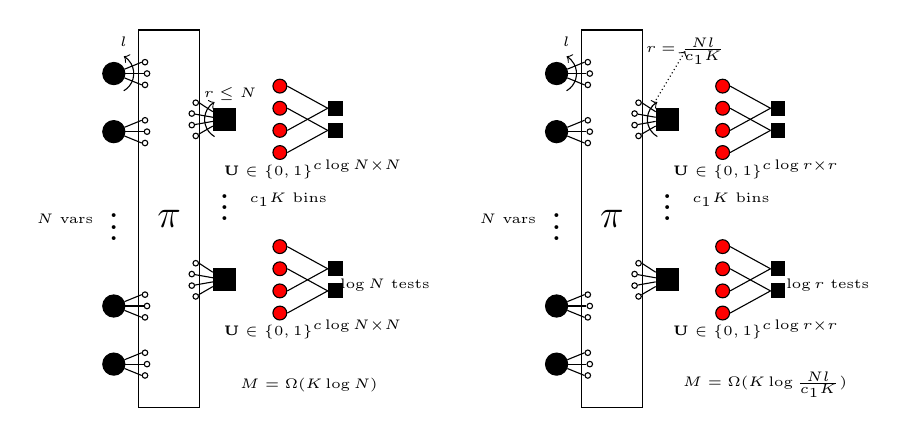
\begin{tikzpicture}
\def\horzgap{40pt}; %Horizontal gap between nodes/levels
\def \gapVN{21pt}; %vertical gap between nodes
\def \gapCN{	29pt}; %Horizontal gap between nodes

\def \textoffs{9pt}; %Offset for writing r\leq N above cn4
\def\nodewidth{8pt};
\def\nodewidthsm{5pt}
\def\edgewidth{2pt};
\def\ext{12pt};
\def\moveX {20pt};
\def\moveYa{4pt}
\def\moveYb{12pt}
\def\arcradius{0.6*\ext}

\def\xmovement{4*\horzgap}

\def \n {8};
\def\ldeg{3};
\def \m {4};
\def\rdeg{6};
\def\langle{40};%120 degrees/3
\def\langle{20};%120 degrees/6

\tikzstyle{check} = [rectangle, draw,  inner sep=0mm, fill=black,minimum height=\nodewidth,minimum width=\nodewidth]
\tikzstyle{checksm} = [rectangle, draw, inner sep=0mm, fill=black,minimum height=\nodewidthsm, minimum width=\nodewidthsm]

\tikzstyle{bit} = [circle, draw, inner sep=0mm, fill=black, minimum size=\nodewidth]
\tikzstyle{bitsm} = [circle, draw, inner sep=0mm,fill=red, minimum size=\nodewidthsm]
\tikzstyle{edgesock} = [circle, inner sep=0mm, minimum size=\edgewidth,draw, fill=white]     

                          
\foreach \vn in {2,3,6,7}{
 \node[bit] (vn\vn) at (0,\vn*\gapVN) {};
\path (vn\vn) ++(20:\ext)node (evA\vn) [edgesock] {};
\path (vn\vn) ++(0:\ext) node (evB\vn) [edgesock] {};
\path (vn\vn) ++(-20:\ext) node (evC\vn) [edgesock] {};

  \draw (vn\vn) -- (evA\vn.west); 
  \draw (vn\vn) -- (evB\vn.west); 
  \draw (vn\vn) -- (evC\vn.west); 
}
\draw[->,thin] (vn7)++(-60:\arcradius) arc (-60:60:\arcradius)node[above]{\tiny{$l$}};

\path (vn3)--node(vndots) {\Large{$\vdots$}} (vn6);
\node[left =-0.2*\nodewidth of vndots](){\tiny{$N$ vars}};

\foreach \cn in {2,4}{
\node[check] (cn\cn) at (\horzgap,0.2in+\cn*\gapCN) {};

\path (cn\cn) ++(150:\ext) node (ecA\cn) [edgesock] {};
\path (cn\cn) ++(170:\ext) node (ecB\cn) [edgesock] {};
\path (cn\cn) ++(190:\ext) node (ecC\cn) [edgesock] {};
\path (cn\cn) ++(210:\ext) node (ecD\cn) [edgesock] {};

  \draw (cn\cn) -- (ecA\cn.east); 
  \draw (cn\cn) -- (ecB\cn);  
  \draw (cn\cn) -- (ecC\cn); 
    \draw (cn\cn) -- (ecD\cn); 
}

\draw[->,thin] (cn4)++(240:\arcradius) arc (240:120:\arcradius);
\path(cn4)++(2pt,\textoffs)node(){\tiny{$r\leq N$}};
\path (cn2)--node(cndots) {\Large{$\vdots$}} (cn4);
\node [right=0.01*\nodewidth of cndots]{\tiny{$c_1K$ bins}};

\node[draw,minimum width=\horzgap-1.5*\ext,minimum height=6.5*\gapVN](perm) at (0.5*\horzgap,4.5*\gapVN){\Large{$\pi$}};

\foreach \cn in {2,4}{
\path (cn\cn) ++(\moveX,\moveYb) node (bitnA\cn) [bitsm] {};
\path (cn\cn) ++(\moveX,\moveYa) node (bitnB\cn) [bitsm] {};
\path (cn\cn) ++(\moveX,-\moveYa) node (bitnC\cn) [bitsm] {};
\path (cn\cn) ++(\moveX,-\moveYb) node (bitnD\cn) [bitsm] {};

\path (bitnB\cn) ++(\moveX,0) node (checknB\cn) [checksm] {};
\path (bitnC\cn) ++(\moveX,0) node (checknC\cn) [checksm] {};

\draw (bitnA\cn.east)--(checknB\cn.west);
\draw (bitnC\cn.east)--(checknB\cn.west);
\draw (bitnB\cn.east)--(checknC\cn.west);
\draw (bitnD\cn.east)--(checknC\cn.west);
\path(bitnD\cn)++(0.6*\moveX,-0.3*\moveX) node(){\tiny{$\mathbf{U}\in\{0,1\}^{c\log N \times N }$}};
}

\path (checknC2)++(2*\textoffs,0.5*\moveYa)node{\tiny{$\log N$ tests}};
\node [below left=3*\nodewidth and 2*\nodewidth of bitnD2,anchor=west]{\tiny{$M=\Omega(K\log N)$} };











\foreach \vn in {2,3,6,7}{
 \node[bit] (Bvn\vn) at (\xmovement,\vn*\gapVN) {};
\path (Bvn\vn) ++(20:\ext)node (BevA\vn) [edgesock] {};
\path (Bvn\vn) ++(0:\ext) node (BevB\vn) [edgesock] {};
\path (Bvn\vn) ++(-20:\ext) node (BevC\vn) [edgesock] {};

  \draw (Bvn\vn) -- (BevA\vn.west); 
  \draw (Bvn\vn) -- (BevB\vn.west); 
  \draw (Bvn\vn) -- (BevC\vn.west); 
}
\draw[->,thin] (Bvn7)++(-60:\arcradius) arc (-60:60:\arcradius)node[above]{\tiny{$l$}};

\path (Bvn3)--node(Bvndots) {\Large{$\vdots$}} (Bvn6);
\node[left =-0.2*\nodewidth of Bvndots](){\tiny{$N$ vars}};

\foreach \cn in {2,4}{
\node[check] (Bcn\cn) at (\xmovement+\horzgap,0.2in+\cn*\gapCN) {};

\path (Bcn\cn) ++(150:\ext) node (BecA\cn) [edgesock] {};
\path (Bcn\cn) ++(170:\ext) node (BecB\cn) [edgesock] {};
\path (Bcn\cn) ++(190:\ext) node (BecC\cn) [edgesock] {};
\path (Bcn\cn) ++(210:\ext) node (BecD\cn) [edgesock] {};

  \draw (Bcn\cn) -- (BecA\cn.east); 
  \draw (Bcn\cn) -- (BecB\cn);  
  \draw (Bcn\cn) -- (BecC\cn); 
  \draw (Bcn\cn) -- (BecD\cn); 
}

\draw[->,thin] (Bcn4)++(240:\arcradius) arc (240:120:\arcradius);
\draw[->,densely dotted](Bcn4)++(140:\arcradius)--++(12pt,20pt)node[](){\tiny{$r=\frac{Nl}{c_1K}$}};
\path (Bcn2)--node(Bcndots) {\Large{$\vdots$}} (Bcn4);
\node [right=0.01*\nodewidth of Bcndots]{\tiny{$c_1K$ bins}};

\node[draw,minimum width=\horzgap-1.5*\ext,minimum height=6.5*\gapVN](Bperm) at (\xmovement+0.5*\horzgap,4.5*\gapVN){\Large{$\pi$}};

\foreach \cn in {2,4}{
\path (Bcn\cn) ++(\moveX,\moveYb) node (BbitnA\cn) [bitsm] {};
\path (Bcn\cn) ++(\moveX,\moveYa) node (BbitnB\cn) [bitsm] {};
\path (Bcn\cn) ++(\moveX,-\moveYa) node (BbitnC\cn) [bitsm] {};
\path (Bcn\cn) ++(\moveX,-\moveYb) node (BbitnD\cn) [bitsm] {};

\path (BbitnB\cn) ++(\moveX,0) node (BchecknB\cn) [checksm] {};
\path (BbitnC\cn) ++(\moveX,0) node (BchecknC\cn) [checksm] {};

\draw (BbitnA\cn.east)--(BchecknB\cn.west);
\draw (BbitnC\cn.east)--(BchecknB\cn.west);
\draw (BbitnB\cn.east)--(BchecknC\cn.west);
\draw (BbitnD\cn.east)--(BchecknC\cn.west);
\path(BbitnD\cn)++(0.6*\moveX,-0.3*\moveX) node(){\tiny{$\mathbf{U}\in\{0,1\}^{c\log r\times r}$}};
}

\path (BchecknC2)++(2*\textoffs,0.5*\moveYa)node{\tiny{$\log r$ tests}};
\node [below left=3*\nodewidth and 2*\nodewidth of BbitnD2,anchor=west]{\tiny{$M=\Omega(K \log \frac{Nl}{c_1K})$} };

\end{tikzpicture}}
\caption{Illustration of the main differences between SAFFRON \cite{lee2015saffron} on the left and our regular-SAFFRON scheme on the right. In both the schemes the peeling decoder on sparse graph requires $\Omega(K)$ bins. But for the bin decoder part, in SAFFRON scheme the right degree is a random variable with a maximum value of $N$ and thus requires $\Omega(\log N)$ tests at each bin. Whereas our scheme based on right-regular sparse graph has a constant right degree of $\Omega(\frac{N}{K})$ and thus requires only $\Omega(\log \frac{N}{K})$ tests at each bin. Thus we can improve the number of tests from $\Omega (K\log N)$ to order optimal $\Omega(K\log \frac{N}{K})$.}
\end{figure*}

\begin{definition}[Regular SAFFRON]
\label{Def:RegSaffron}
We define the ensemble of testing matrices for our scheme to be $\mc{G}_{\ell,r}(N,M_1)\times \mbf{U}_{r,p}$ where a graph $G$ is chosen from $\mc{G}_{\ell,r}(N,M_1)$, a signature matrix $\mbf{U}$ is chosen from $\mbf{U}_{r,p}$ and the testing matrix is defined according to Eq. \eqref{Eqn:TestingMatrixDefn}. Note that the total number of tests for this testing scheme is $(2p+2)M_1\log r$ where $r=\frac{N\ell}{M_1}$.
\end{definition}

For the regular SAFFRON testing ensemble defined in Def. \ref{Def:RegSaffron}, we employ the same peeling based decoder described in Sec.~\ref{Sec:PriorWork}. 

Now we consider the performance analysis of the regular SAFFRON scheme under the peeling based decoder. Similar to the SAFFRON scheme we will analyze the peeling decoder and the bin decoder separately and union bound the total error probability of the decoding scheme. As we have already mentioned the analysis of the peeling decoder part alone can be carried out by considering a \textit{simplified oracle-based peeling decoder} on a pruned graph with only the non-zero variable nodes remaining. 

\begin{definition}[Pruned graph ensemble]
We will define the pruned graph ensemble $\tilde{\mc{G}}_{\ell,r}(N,K,M_1)$ as the set of all graphs obtained from removing a random $N-K$ subset of variable nodes from a graph from the ensemble $\mc{G}_{\ell,r}(N,M_1)$.
\end{definition}

Note that graphs from the pruned ensemble have $K$ variable nodes with a degree $\ell$ whereas the right degree is not regular anymore. 

\begin{lemma}[Edge d.d of pruned graph]
\label{Lem:EdgeDDPrunedGraph}
For the pruned graph ensemble $\tilde{\mc{G}}_{\ell,r}(N,K,M_1)$ it can be shown in the limit $K,N\rightarrow\infty$ that edge d.d coefficients $\rho_{1}=e^{-\lambda}$ and $\rho_{2}=\lambda e^{-\lambda}$ where $\lambda=\ell/c_1$ for the choice of $M_1=c_1K$, $c_1$ being some constant.
\end{lemma}

Note that even if our initial ensemble is left-and-right-regular the pruned graph has asymptotically same degree distribution as in the SAFFRON scheme where the initial graph is from left-regular ensemble.

\begin{lemma}
\label{Lem:PeelingRegularAnalysis}
For the pruned graph ensemble $\tilde{\mc{G}}_{\ell,r}(N, K,M_1)$ the oracle-based peeling decoder fails to peel off atleast $(1-\epsilon)$ fraction of the variable nodes with exponentially decaying probability for $M_1=c_1(\epsilon)K$ where $c_1(\epsilon)$ for various $\epsilon$ is given in Table. \ref{Table:constantsDE}.
\end{lemma}


\begin{proof}
From Lemma. \ref{Lem:EdgeDDPrunedGraph} we know that the edge degree distribution coefficients $\rho_1$ and $\rho_2$ are identical to that of the SAFFRON scheme and hence the same DE equations can be used here. Therefore the exact same proof as the proof of Lemma. \ref{Lem:PeelingAnalysisLeftRegular} can be employed here.
\end{proof}

\begin{theorem}
\label{Thm:NoiselessMain}
Let $p\in\Z$ such that $K$ and $N$ scale as $K\in o(N^{\frac{p}{p+1}})$. For $M=(2p+2)c_1(\epsilon)K \log_{2}\frac{N}{K}$, the regular SAFFRON framework we proposed, asymptotically, recovers atleast a $(1-\epsilon)$ fraction of the defective items for arbitrarily-small $\epsilon$ with high probability $1-O\left(\frac{K^{p+1}}{N^p}\right)$. Note that computational complexity of the decoding scheme is $O(K\log \frac{N}{K})$. The constant $c_1(\epsilon)$ is given in Table. \ref{Table:constantsDE}.
\end{theorem}
\begin{proof}
It remains to be shown that the total probability of error decays asymptotically in $K$ and $N$. Let $E_1$ be the event of oracle-based peeling decoder terminating without recovering atleast $(1-\epsilon)K$ variable nodes. Let $E_2$ be the event of the bin decoder making an error during the entirety of the peeling process and $E_{\tx{bin}}$ be the event of one instance of bin decoder making an error. The total probability of error $P_e$ can be upper bounded by 
\begin{align*}
P_e &\leq \tx{Pr}(E_1)+ \tx{Pr}(E_2)\\
               &\leq \tx{Pr}(E_1)+ K\ell\tx{Pr}(E_{\tx{bin}})\\
               &\in O\left(\frac{K^{p+1}}{N^p}\right)
\end{align*}
where the second inequality is due to the union bound over a maximum of $Kl$ instances of bin decoding. The third line is due to the fact that $\tx{Pr}(E_1)$ is exponentially decaying in $K$ (see Lemma. \ref{Lem:PeelingRegularAnalysis}) and $\tx{Pr}(E_{\tx{bin}})=(\frac{c_1K}{N\ell})^p$ (see Lemma. \ref{Lem:BinDecoderAnalysis} and Def. \ref{Def:RegSaffron})
\end{proof}

\begin{proof}[Proof of Lem. \ref{Lem:EdgeDDPrunedGraph}]
We will first derive $R(x)$ for the pruned graph ensemble and then use the relation\cite{richardson2008modern} $\rho(x)=\frac{R'(x)}{R'(1)}$ to derive the edge d.d . Note that all the check nodes have a uniform degree $r$ before pruning. When pruning we are removing a $N-K$ subset of variable nodes at random i.e., asymptotically this is equivalent to removing each edge from the graph with a probability $1-\epsilon$ where $\epsilon\coleq \frac{K}{N}$. Under this process the right-node d.d can be written as
\begin{align}
R_1&=r\epsilon(1-\epsilon)^{r-1},\quad \text{ and similarly}\label{Eqn:Deg1ChkDistribution}\\
R_i &=\binom{r}{i} \epsilon^{i}(1-\epsilon)^{r-i},\nonumber
\end{align}
thus giving us $R(x)=(\epsilon x+(1-\epsilon))^{r}$. This gives us 
\begin{align*}
\rho(x)&=\frac{r\epsilon(\epsilon x+(1-\epsilon))^{r-1}}{r\epsilon}\\
          &=(\epsilon x+(1-\epsilon))^{r-1}.
\end{align*}
Thus we can compute that $\rho_1=(1-\epsilon)^{r-1}$ and $\rho_2=(r-1)\epsilon(1-\epsilon)^{r-2}$. We evaluate these quantities asymptotically as $K,N\rightarrow \infty$ and $M_1=CK$.
\begin{align*}
\lim_{K,N\rightarrow \infty} \rho_1&=\lim_{K,N\rightarrow \infty} (1-\frac{K}{N})^{\frac{Nl}{CK}-1}\\
&=e^{-\lambda} \qquad \text{ where } \lambda=\frac{l}{C}
\end{align*}
Similarly we can show $\lim_{K,N\rightarrow \infty}\rho_2=\lambda e^{-\lambda}$.
\end{proof}


\section{Total recovery: Singleton-Only Variant}
In this section we will look at the proposed regular-SAFFRON scheme but with a decoder that uses only the singleton bins. To elaborate the only difference is in the decoder, which is not iterative in this scheme, recovers the variable nodes connected to all the degree-1 check nodes and terminates. We will refer to this scheme as \textit{singleton-only} regular-SAFFRON scheme. The downside of this using this scheme, even though we can now recover the \textit{whole} defective set instead of just a large fraction of the defective items, is that now the left-degree of the bipartite graph, or equivalently the number of times a sample is divided for testing, cannot be finite and needs to be scaled as $\log K$.

Since we do not need to be able to recover resolvable double-tons we only need $2\log_2 r$ number of tests at each bin i.e. $p=0$ in Eqn. \eqref{Eqn:SignatureMatrix}.
\begin{theorem}
Using a $(\ell,r)=(c_\alpha \log K,\frac{N}{K})$ regular-bipartite graph, the regular-SAFFRON scheme with $m=2c_\alpha K\log K \log_2 \frac{N}{K}$ tests and the singleton-only decoder fails to recover all the non-zero variable nodes with a vanishing probability of $O(\frac{1}{K^{\alpha}})$ where $c_\alpha=e(1+\alpha)$.
\end{theorem}
\begin{proof}
As the number of tests in each bin is $2\log_2 \frac{N}{K}$ it is enough if we show that for the number of bins in the bipartite graph equal to $e(1+\alpha)K\log K$ all the variable nodes in the pruned graph are connected to atleast one singleton bin with high probability.

In the pruned graph ensemble, for any particular variable node, the probability that any of the $\ell$ connected bit nodes are not a singleton can be given by $(1-R_1)^\ell$ where $R_1$ is the probability that a bin node in the pruned graph ensemble is a singleton. From Eq. \ref{Eqn:Deg1ChkDistribution} asymptotically the value of $R_1$ approaches 
\begin{align*}
R_1&=\lim _{K,N\rightarrow\infty}r\epsilon(1-\epsilon)^{r-1}\\
     &=\lim _{K,N\rightarrow\infty}\left(1-\frac{K}{N}\right)^{\frac{N}{K}-1}\\
     &\approx e^{-1}
\end{align*} 
By using union bound over all the $K$ variable nodes in the pruned graph, the probability $P_e$ that the singleton-only decoder fails to recover a defective item can be bounded by
\begin{align*}
P_e&\leq K(1-R_1)^\ell \\
&=K\left(1-e^{-1}\right)^{e(1+\alpha)\log K}\\
&\leq Ke^{-e^{-1}e(1+\alpha)\log K}\\
&=K^{-\alpha},
\end{align*}
where for the third inequality we employ $(1-x)\leq e^{-x}$
\end{proof}


\section{Robust Group Testing}
\label{Sec:NoisyGroupTesting}
In this section we extend our scheme to the group testing problem where the test results can be noisy. To be formal, the signal model looks like
\begin{align*}
\mbf{y=A}\odot \mbf{x+w},
\end{align*}
where the addition is over binary field and $\mbf{w}\in\{0,1\}^N$ is an i.i.d noise vector distributed according to Bernoulli distribution with parameter $0<q<\frac{1}{2}$.

\subsection*{Testing Scheme}
In \cite{lee2015saffron} for the robust group testing problem, the signature matrix used for noiseless group testing problem is modified using a error control coding such that it can handle singletons and resolvable doubletons in the presence of noise. The binning operation as defined by the bipartite graph is exactly identical to that of noiseless case. We describe the modifications to the signature matrix and the bin detection decoding scheme as given in \cite{lee2015saffron} for the sake of completeness and then state the performance bounds for our scheme for the noisy group testing problem.

Let $\mc{C}_n$ be a binary error-correcting code with the following definition:
\begin{itemize}
\item Let the encoder and decoder functions be $f:\{0,1\}^{n}\rightarrow \{0,1\}^{\frac{n}{R}}$ and $g:\{0,1\}^{\frac{n}{R}}\rightarrow \{0,1\}^{n}$ respectively where $R$ is the rate of the code.
\end{itemize}
We can use any error-correcting code but for ease of analysis and tight upper bound for the number of tests we will use spatially-coupled LDPC codes which are known to be capacity achieving \cite{kumar2014threshold,kudekar2013spatially}. For spatially-coupled LDPC codes, being capacity achieving is equivalent to: 
\begin{itemize}
\item There exists a sequence of codes $\{\mc{C}_n\}$ with the rate of each code being $R$ satisfying 
\begin{align}
\label{Eqn:ProbErrorCoding}
R<1-H(q)-\delta=1+q\log_2 q+ \overline{q}\log_2\overline{q}-\delta
\end{align}
for any arbitrary small constant $\delta$ such that the probability of error $\text{Pr}\left(g(\mbf{x+w})\neq \mbf{x}\right)<2^{-\kappa n}$ for some $\kappa >0$. In Eqn.~\ref{Eqn:ProbErrorCoding}, $\overline{q}\coleq 1-q$. 
\end{itemize} 
The modified signature matrix $\mbf{U}'_{r,p}$ can be described via $\mbf{U}_{r, p}$ given in Eq. \eqref{Eqn:SignatureMatrix}, and encoding function $f$ for a code $\mc{C}_{\log_2 r}$ as follows:
 \begin{align}
\label{Eqn:SignatureMatrixModified}
\mbf{U}_{r,p}'\coleq\begin{bmatrix}
f(\mbf{b}_1)  & f(\mbf{b}_2) &\cdots & f(\mbf{b}_r) \\
\overline{f(\mbf{b}_1)} & \overline{f(\mbf{b}_2)} & \cdots & \overline{f(\mbf{b}_r)}\\
f(\mbf{b}_{\pi^{1}_{1}}) & f(\mbf{b}_{\pi^{1}_{2}}) & \cdots & f(\mbf{b}_{\pi^{1}_{r}})\\
\overline{f(\mbf{b}_{\pi^{1}_{1}})} & \overline{f(\mbf{b}_{\pi^{1}_{2}})} & \cdots & \overline{f(\mbf{b}_{\pi^{1}_{r}})}\\
\cdots &  &\vdots \\
f(\mbf{b}_{\pi^{p}_{1}}) & f(\mbf{b}_{\pi^{p}_{2}}) & \cdots & f(\mbf{b}_{\pi^{p}_{r}})\\
\overline{f(\mbf{b}_{\pi^{p}_{1}})} & \overline{f(\mbf{b}_{\pi^{p}_{2}})} & \cdots & \overline{f(\mbf{b}_{\pi^{p}_{r}})}\\
\end{bmatrix}
\end{align}  
Then the overall testing matrix $\mbf{A}$ is defined in identical fashion to the definition in Sec. \ref{Sec:PriorWork} for the case of noiseless case except that $\mbf{U}$ will be replaced by $\mbf{U'}$ in Eqn.~\eqref{Eqn:SignatureMatrixModified}. Formally it can be defined as $\mbf{A}\coleq [\mbf{A}_{1}^{T},\ldots,\mbf{A}_{M_{1}}^{T}]^T$ where $\mbf{A}_{i}=\mbf{U'} \diag (\mbf{t}_i)$ where the binary vectors $\mbf{t}_i$ are defined in Sec. \ref{Sec:PriorWork}. 

\subsection*{Decoding}
The decoding scheme for the robust group testing, similar to the case of noiseless case, has two parts with the iterative peeling part of the decoder identical to that of the noiseless case whereas the bin detection part differs slightly with an extra step of decoding for the error control code involved.

Given the test output vector at a bin $\mbf{y}=[\mbf{y}^{T}_{01},\mbf{y}^{T}_{02},\mbf{y}^{T}_{11},\ldots,\mbf{y}^{T}_{p2}]^T$, the bin detection for the noisy case can be summarized as following: The decoder first applies the decoding function $g(\cdot)$ to the first segments in each section $\mbf{y}_{i1} \forall i\in[0:p]$ then obtains the locations $l_0,l_1,\ldots l_p$ whose binary expansions are equal to the error-correcting decoder outputs $g(\mbf{y}_{i1})$. The decoder declares the bin as a singleton if $\pi_{l_0}^{i}=l_i~\forall i$.

Similarly given that one of the variable nodes connected to the bin is already decoded to be non-zero, the resolvable double-ton decoding can be summarized as following. Let the location of the already recovered variable node in the bin (originally a double-ton) be $l_0$ then the test output can be given as 
\begin{align*}
\begin{bmatrix}
\mbf{y}_{01}\\
\mbf{y}_{02}\\
\mbf{y}_{11}\\
\vdots \\
\mbf{y}_{p2}\\
\end{bmatrix}
=\mbf{u}_{l_0} \vee \mbf{u}_{l_1}+\mbf{w}=
\begin{bmatrix}
f(\mbf{b}_{l_0})\\
\vspace{2pt}
\overline{f(\mbf{b}_{l_0})}\\
f(\mbf{b}_{\pi^1_{l_0}})\\
\vdots \\
\overline{f(\mbf{b}_{\pi^p_{l_0}})}\\
\end{bmatrix} 
\vee
\begin{bmatrix}
f(\mbf{b}_{l_1})\\
\vspace{2pt}
\overline{f(\mbf{b}_{l_1})}\\
f(\mbf{b}_{\pi^1_{l_1}})\\
\vdots \\
\overline{f(\mbf{b}_{\pi^p_{l_1}})}\\
\end{bmatrix}+
\begin{bmatrix}
\mbf{w}_{01}\\
\vspace{2pt}
\mbf{w}_{02}\\
\mbf{w}_{11}\\
\vdots \\
\mbf{w}_{p2}\\
\end{bmatrix}
\end{align*} 
where the location of the second non-zero variable node $l_1$ needs to be recovered. Given $\mbf{y}=\mbf{u}_{l_0} \vee \mbf{u}_{l_1}+\mbf{w}$ and $\mbf{u}_{l_0}$, $\mbf{u}_{l_1}+\mbf{w}$ can be recovered since for each segment of $\mbf{u}_{l_0}$ either the vector $f(\mbf{b}_{\pi^k_{l_0}})$ or it's complement is available. Once $f(\mbf{b}_{\pi_{l_1}^i})+\mbf{w}$ is recovered for each segment $i$, we apply singleton decoding procedure and rules as described above.

\begin{figure}[t!]
\centering
\resizebox{\columnwidth}{!}{\input{./Figures/noiseless_Kannan.tex}}
\caption{MonteCarlo simulations for $K=100, N=2^{16}$. We compare the SAFFRON scheme with our regular SAFFRON scheme for various left degrees $\ell\in\{3,5,7\}$. For a given $\ell$ the bin detection size is fixed and we vary the number of bins. The plots in blue indicate the SAFFRON scheme and the plots in red indicate our regular SAFFRON scheme based on left-and-right-regular bipartite graphs.}
\label{Fig:SimulationNoiseless}
\end{figure}

\begin{lemma}[Robust Bin Decoder Analysis]
For a signature matrix $\mbf{U'}_{r,p}$ as described in \eqref{Eqn:SignatureMatrixModified}, the robust bin decoder misses a singleton with probability no greater than $\frac{p+1}{r^{\kappa}}$. The robust bin decoder wrongly declares a singleton with probability no greater than $\frac{1}{r^{p+\kappa}}$.
\end{lemma}
The fraction of missed singletons will be compensated by using $M(1+\frac{p+1}{r^{\kappa}})$ instead of $M$ such that the total number of singletons decoded will be $M(1+\frac{p+1}{r^{\kappa}})(1-\frac{p+1}{r^{\kappa}})\approx M$.

\begin{theorem}
Let $p\in\Z$ such that $K$ and $N$ scale as $K\in o\left(N^{\frac{p}{p+1}}\right)$
% where $\kappa>0$ is defined in Eq. \eqref{Eqn:ProbErrorCoding}
. For $M=2(p+1)\beta(q)c_1(\epsilon)K \log_{2}\frac{N}{K}$, the robust regular SAFFRON framework we proposed, asymptotically, recovers atleast a $(1-\epsilon)$ fraction of the defective items for arbitrarily-small $\epsilon$ with high probability $1-O\left(\frac{K^{p+\kappa+1}}{N^{p+\kappa}}\right)$. Here $\beta(q)=\frac{1}{R}>\frac{1}{1-H(q)-\delta}$ for an arbitrary small constant $\delta$ and the constants $c_1(\epsilon)$ are given in Table. \ref{Table:constantsDE}. Note that computational complexity of the decoding scheme is $O(K\log \frac{N}{K})$.
\end{theorem}

\section{Simulation Results}
In this section we will evaluate the performance of our proposed regular SAFFRON scheme via Monte Carlo simulations and compare it with the results for SAFFRON scheme provided in \cite{lee2015saffron}.

\subsection*{Noiseless Group Testing}
As per Thm.~\ref{Thm:NoiselessMain} the regular SAFFRON scheme we proposed recovers $(1-\epsilon)$ fraction of defective items with a high probability for $M_1>c_1 K$ where the pairs ($c_1,\ell$) are given for various values of error floors $\epsilon$ in Table.~\ref{Table:constantsDE}. We demonstrate this by simulating the performance for the system parameters summarized below.
\begin{itemize}
\item We fix $N=2^{16}$ and $K=100$
\item In Eqn.~\ref{Eqn:SignatureMatrix} the parameter $p=2$ is chosen i.e. $h=6\log_2 r$
\item For $\ell\in\{3,5,7\}$ we vary the number of bins $M_1=cK$. 
\item Hence the total number of tests $M=6cK\log_2 \left(\frac{N\ell}{cK}\right)$
\end{itemize} 
The results are shown in Fig.~\ref{Fig:SimulationNoiseless}. We observe that there is clear improvement in performance for our regular SAFFRON scheme when compared to the SAFFRON scheme for each $\ell\in\{3,5,7\}$.

\begin{figure}[t!]
\centering
% This file was created by matlab2tikz v0.4.7 running on MATLAB 7.14.
% Copyright (c) 2008--2014, Nico Schlömer <nico.schloemer@gmail.com>
% All rights reserved.
% Minimal pgfplots version: 1.3
% 
% The latest updates can be retrieved from
%   http://www.mathworks.com/matlabcentral/fileexchange/22022-matlab2tikz
% where you can also make suggestions and rate matlab2tikz.
% 
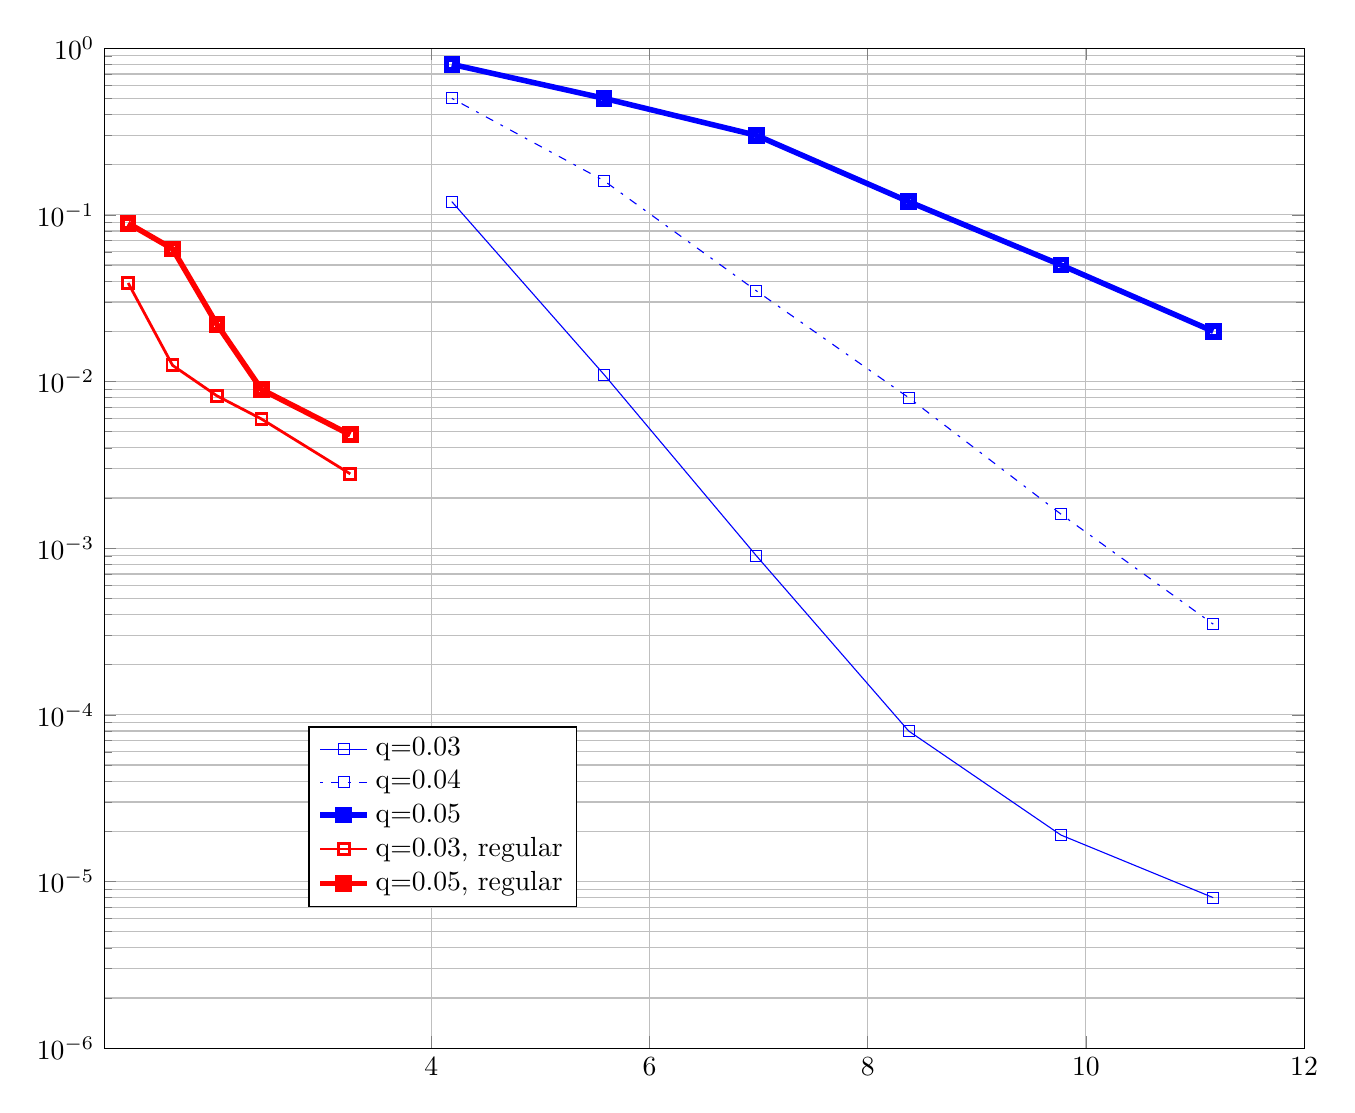
\begin{tikzpicture}

\begin{axis}[%
width=6.0in,
height=5.0in,
scale only axis,
xmin=1,
xmax=12,
xmajorgrids,
xtick = {4,6,8,10,12},
ymode=log,
ymin=1e-06,
ymax=1,
yminorticks=true,
ymajorgrids,
yminorgrids,
legend style={at={(0.170351155044956,0.141495348339839)},anchor=south west,draw=black,fill=white,legend cell align=left}
]
\addplot [color=blue,solid,mark=square,mark options={solid}]
  table[row sep=crcr]{4.1877504	 0.12\\
5.5836672	0.011\\
6.979584 	0.0009\\
8.3755008	8e-05\\
9.7714176	1.9e-05\\
11.1673344	 8e-06\\
};
\addlegendentry{q=0.03};

\addplot [color=blue,dash pattern=on 1pt off 3pt on 3pt off 3pt,mark=square,mark options={solid}]
  table[row sep=crcr]{4.1877504 	0.5\\
5.5836672		0.16\\
6.979584 		0.035\\
8.3755008		0.008\\
9.7714176	 	0.0016\\
11.1673344 	0.00035\\
};
\addlegendentry{q=0.04};

\addplot [color=blue,solid,line width=2.0pt,mark=square,mark options={solid}]
  table[row sep=crcr]{4.1877504 	0.8\\
5.5836672		0.5\\
6.979584 		0.3\\
8.3755008		0.12\\
9.7714176		0.05\\
11.1673344 	0.02\\
};
\addlegendentry{q=0.05};

\addplot [color=red,solid,line width=1.0pt,mark=square,mark options={solid}]
  table[row sep=crcr]{1.221 	3.90e-2\\
   1.628  	1.25e-2\\
   2.035	8.2e-3\\
   2.443	5.96e-3\\
   3.257	2.79e-3  \\
};
\addlegendentry{q=0.03, regular};


\addplot [color=red,solid,line width=2.0pt,mark=square,mark options={solid}]
  table[row sep=crcr]{1.221 	8.90e-2\\
   1.628  	6.25e-2\\
   2.035	2.2e-2\\
   2.443	8.96e-3\\
   3.257	4.79e-3  \\
};
\addlegendentry{q=0.05, regular};

\end{axis}
\end{tikzpicture}
%\resizebox{\columnwidth}{!}{}
\caption{MonteCarlo simulations for $K=128, N=2^{32}$. We compare the SAFFRON scheme with our regular SAFFRON scheme for a left degree $\ell=12$. We fix the number of bins and vary the rate of the error control code used. The plots in blue indicate the SAFFRON scheme\cite{lee2015saffron} and the plots in red indicate our regular SAFFRON scheme based on left-and-right-regular bipartite graphs.}
\label{Fig:SimulationNoisy}
\end{figure}


\subsection*{Noisy Group Testing}
Similar to the noiseless group testing problem we simulate the performance of our regular SAFFRON scheme and compare it with that of the SAFFRON scheme. For convenience of comparison we choose our system parameters identical to the choices in \cite{lee2015saffron}. The system parameters can be summarized as follows:
\begin{itemize}
\item $N=2^{32}, K=2^7$. We choose  $\ell=12, M_1=11.36K$ 
\item Hence the total number of tests is $M=6cK\log_2 \left(\frac{N\ell}{cK}\right)$
\item We simulate for BSC noise parameter $q\in\{0.03,0.04,0.05\}$
\end{itemize}
For the signature matrix we choose $p=1$ in Eqn.~\ref{Eqn:SignatureMatrix} i.e. $h=4\log_2 r$. Note that for the above set of parameters the right degree $r=\frac{N\ell}{M_1}\approx 26$. By choosing to operate in field $GF(2^7)$ gives us a message of length $4$ symbols. Then we encode using a $(4+2e,4)$ Reed-Solomon code for $e\in[0:8]$ thus giving us a column length of $4\times 7(4+2e)$ bits.
\bibliographystyle{ieeetr}
\bibliography{\MyPath/journal_abbr,\MyPath/sparseestimation,grouptesting}
\end{document} 
